\section{Result}
\begin{figure}[H]
\centering
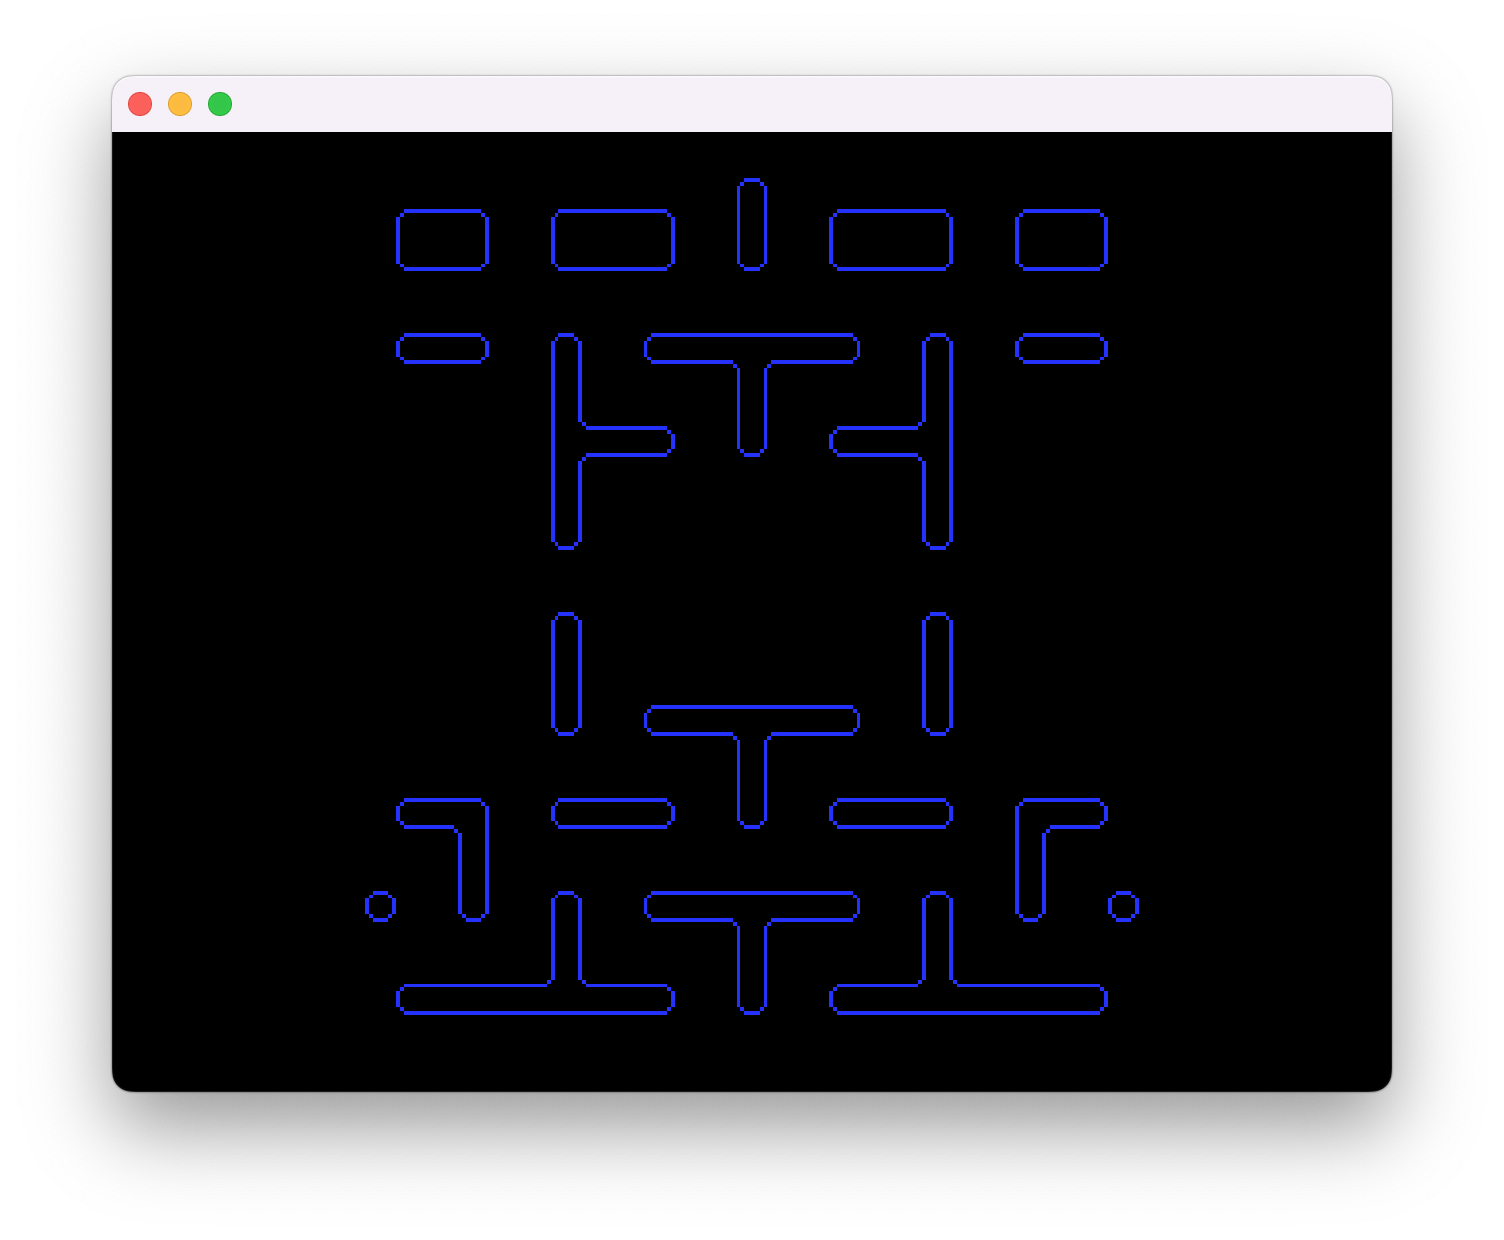
\includegraphics[width=0.8\linewidth]{Image-8.png}
\caption {Output of first algorithm\autocite{myself}}\label{FirstOutput}
\end{figure}

\section{Analysis of Algorithm 1}
Algorithms run at speeds related to the number of operations that it must make, based on an input of a certain size. This is described by the big-O notation $O(f(x))$ where $f(x)$ is a function relating the input size to the steps the algorithm must make. Our algorithm, applied to a square lattice graph of a boundary customary to Pac-Man will step on each tile exactly once, and at each tile will check at most 3 directions (all cardinal directions except for the one we walked from). Thus if we let the input size $n$ be the number of tiles in a wall boundary, then we have a speed of $O(3n)$, also refered to as linear-time complexity, meaning that as the input size increases linearly, the time taken by the algorithm will, in the worst case, change proportionally to that, which is considered efficient. 

\section{Limitations of Algorithm 1}
Figure ~\ref{FirstOutput}, shows the algorithm applied to the original Pac-Man level. Most of the tiles are colored, yet the image is missing the tiles forming the boundary of the level, when comparing with Figure ~\ref{PacmanLevelGrid}. This is because the outer boundary is fundamentally different from the central ones. 
The $Normal(d)$ function which lies at the center of deciding in what direction our Hamiltonian cycle must go is in fact reversed. 